% SutureAI platform user guide (warm-paper edition, matches the redesigned app).
% Build (from docs/user-guide):
%   python ../design/tools/prepare-fonts.py build/fonts   # Barlow TTFs from node_modules
%   latexmk -xelatex -outdir=build sutureai-user-guide.tex
% Screenshots: node tools/capture-screenshots.mjs <baseUrl> <demo-video>  (see that file's header)
\documentclass[11pt,a4paper]{article}

\usepackage[margin=2.2cm,top=2.4cm,bottom=2.4cm]{geometry}
\usepackage{fontspec}
\usepackage{xcolor}
\usepackage{graphicx}
\usepackage{tikz}
\usetikzlibrary{arrows.meta,positioning,fit,backgrounds,calc}
\usepackage{booktabs,tabularx,array,colortbl}
\usepackage{enumitem}
\usepackage[most]{tcolorbox}
\usepackage{titlesec}
\usepackage{fancyhdr}
\usepackage{caption}
\usepackage{fontawesome5}
\usepackage[hidelinks]{hyperref}
\usepackage{float}
\usepackage{needspace}
\usepackage{hyphenat}

\newcolumntype{L}[1]{>{\raggedright\arraybackslash}p{#1}}
\newcolumntype{Y}{>{\raggedright\arraybackslash}X}

% ---- fonts (the app's own pair) --------------------------------------------------
\setmainfont{Montserrat-Regular.otf}[
  BoldFont=Montserrat-SemiBold.otf,
  ItalicFont=Montserrat-Italic.otf,
  BoldItalicFont=Montserrat-SemiBoldItalic.otf]
\setmonofont{SourceCodePro-Regular.otf}[Scale=0.92]
\newfontfamily\display{Barlow-SemiBold.ttf}[Path=build/fonts/, BoldFont=Barlow-Bold.ttf]
\newfontfamily\cjk{Microsoft YaHei}

% ---- palette (matches tailwind.config.js) ------------------------------------------
\definecolor{paper}{HTML}{F8F6F1}
\definecolor{tile}{HTML}{F2EFE9}
\definecolor{line}{HTML}{E8E3D8}
\definecolor{mist}{HTML}{D9D3C6}
\definecolor{ink}{HTML}{2B2924}
\definecolor{inksoft}{HTML}{4A463F}
\definecolor{muted}{HTML}{6F6A60}
\definecolor{brand}{HTML}{4F69C2}
\definecolor{brandfifty}{HTML}{F1F4FC}
\definecolor{brandtwo}{HTML}{C5D1F0}
\definecolor{brandthree}{HTML}{9DB0E3}
\definecolor{brandsix}{HTML}{3F57A8}
\definecolor{brandeight}{HTML}{26365F}
\definecolor{good}{HTML}{4A7456}
\definecolor{warn}{HTML}{8C6A22}
\definecolor{bad}{HTML}{A24E36}

\pagecolor{paper}
\color{ink}
\hypersetup{colorlinks=true,linkcolor=brand,urlcolor=brand}
\setlength{\parindent}{0pt}
\setlength{\parskip}{0.55em}
\linespread{1.08}
\setlist{itemsep=0.15em,topsep=0.3em}
\arrayrulecolor{mist}
\renewcommand{\arraystretch}{1.2}

% Section labels follow the app: blue two-digit number, Barlow title.
\titleformat{\section}{\Needspace{10\baselineskip}\display\LARGE\bfseries\color{brandeight}}{\color{brand}\normalsize\thesection\hspace{0.35em}}{0.4em}{}
\titleformat{\subsection}{\Needspace{6\baselineskip}\display\Large\color{brandeight}}{\color{brand}\small\thesubsection}{0.6em}{}
\titlespacing*{\section}{0pt}{1.8em}{0.6em}
\titlespacing*{\subsection}{0pt}{1.2em}{0.35em}
\makeatletter\renewcommand{\thesection}{\two@digits{\value{section}}}\makeatother

\captionsetup{font={small,color=muted},labelfont={bf,color=muted},skip=6pt}

\pagestyle{fancy}
\fancyhf{}
\renewcommand{\headrulewidth}{0pt}
\fancyhead[L]{\small\color{muted}SutureAI · User Guide}
\fancyhead[R]{\small\color{muted}\leftmark}
\fancyfoot[C]{\small\color{muted}\thepage}
\renewcommand{\sectionmark}[1]{\markboth{#1}{}}

% ---- helpers -------------------------------------------------------------------
\newcommand{\ui}[1]{\textbf{\color{brand}\nohyphens{#1}}} % a button / control (never hyphenated)
\newcommand{\page}[1]{\leavevmode{\ttfamily\small\color{brandeight}#1}} % a route
\newcommand{\sect}[2]{{\color{brand}\small #1}\,\emph{#2}} % a numbered section of a page
\newlength{\shotmax}\setlength{\shotmax}{0.38\textheight}  % tallest a screenshot may be
\newcommand{\shot}[3][\linewidth]{%                      % screenshot with hairline frame
  \begin{figure}[H]\centering
  \fcolorbox{line}{white}{\includegraphics[width=\dimexpr#1-2\fboxsep-2\fboxrule\relax,
    height=\shotmax,keepaspectratio]{figures/#2}}
  \caption{#3}\end{figure}}

% Grey tile, dashed tile and blue tile, as in the app.
\newtcolorbox{tilebox}[1][]{enhanced, colback=tile, colframe=tile, boxrule=0pt, arc=4pt,
  left=10pt,right=10pt,top=8pt,bottom=8pt, fontupper=\small, #1}
\newtcolorbox{dashedbox}[1][]{enhanced, colback=tile, frame hidden, arc=4pt,
  borderline={0.8pt}{0pt}{brandthree,dashed}, left=10pt,right=10pt,top=8pt,bottom=8pt, fontupper=\small, #1}
\newtcolorbox{bluebox}[1][]{enhanced, colback=brandfifty, colframe=brandfifty, boxrule=0pt, arc=4pt,
  left=10pt,right=10pt,top=8pt,bottom=8pt, fontupper=\small, #1}
\newcommand{\tiletitle}[2][brand]{{\display\large\color{brandeight}\textcolor{#1}{\raisebox{0.15ex}{\tikz\fill (0,0) circle (2.4pt);}}\hspace{0.45em}#2}\par\smallskip}

% Tips are blue tiles, notes are grey tiles with an ochre dot.
\newenvironment{tip}{\begin{bluebox}[before skip=8pt, after skip=8pt]\tiletitle{Tip}}{\end{bluebox}}
\newenvironment{note}[1][Note]{\begin{tilebox}[before skip=8pt, after skip=8pt]\tiletitle[warn]{#1}}{\end{tilebox}}

% Outlined, square-cornered chip (severity, status), as in the app.
\newtcbox{\chip}[1][brand]{on line, enhanced, colback=white, colframe=#1!70, coltext=#1,
  boxrule=0.5pt, arc=0pt, left=3pt, right=3pt, top=1pt, bottom=1pt, fontupper=\scriptsize\bfseries}

\tikzset{
  box/.style={draw=#1,fill=white,rounded corners=3pt,line width=0.7pt,align=center,
              minimum height=1.05cm,text width=2.2cm,font=\small,text=ink},
  box/.default=brand,
  arr/.style={-{Stealth[length=2.2mm]},line width=0.7pt,color=muted},
  lane/.style={rounded corners=5pt,inner sep=7pt},
  lanelabel/.style={font=\scriptsize\bfseries,color=muted,anchor=south west,inner sep=2pt},
  state/.style={draw=#1,fill=white,rounded corners=2pt,line width=0.7pt,font=\small\ttfamily,
                text=#1,minimum height=0.8cm,inner xsep=7pt},
  state/.default=brand,
}

\begin{document}

% ---- title ---------------------------------------------------------------------
\thispagestyle{empty}
\begin{tikzpicture}[remember picture,overlay]
  \fill[brand] (current page.north west) rectangle ([yshift=-0.35cm]current page.north east);
\end{tikzpicture}
\vspace*{1.6cm}
{\small\color{muted}SUTUREAI \textperiodcentered\ USER GUIDE \textperiodcentered\ PROTOTYPE EDITION}\par
\vspace{0.35cm}
{\display\fontsize{38}{42}\selectfont\bfseries\color{brandeight}Platform User Guide}\par
\vspace{0.25cm}
{\Large\color{inksoft}Recording, scoring and reviewing simulated suturing practice}\par
\vspace{0.2cm}
{\small\color{muted}For students and instructors \textperiodcentered\ October 2026}\par
\vspace{0.6cm}

% Stitched incision, the product's ornament.
\begin{tikzpicture}[x=0.046cm,y=-0.046cm]
  \draw[brandtwo, line width=1.1pt, line cap=round] (10,70) .. controls (70,30) and (130,95) .. (190,55) .. controls (250,15) and (300,30) .. (350,60);
  \foreach \a/\b/\c/\d [count=\i, evaluate=\i as \op using 0.45+0.06*\i] in {38/42/50/70, 76/46/84/72, 114/56/120/82, 152/58/156/84, 190/44/192/70, 228/34/232/60, 266/30/272/56, 304/38/312/62}
    \draw[brand, line width=1.1pt, line cap=round, opacity=\op] (\a,\b) -- (\c,\d);
\end{tikzpicture}

\vspace{0.6cm}
\begin{tcolorbox}[enhanced, colback=white, colframe=line, boxrule=0.5pt, arc=4pt, left=12pt, right=12pt, top=10pt, bottom=10pt]
\small
\textbf{What SutureAI does.} Students record a practice task (simple suturing, knot tying or
needle handling) and upload the video. The platform scores it on five dimensions and writes a
report that links each finding to a moment in the video. Instructors follow their whole class,
confirm or adjust scores, and decide students' appeals against individual findings.

\medskip
\begin{tabularx}{\linewidth}{@{}>{\leavevmode\color{brand}}l >{\bfseries}l Y@{}}
\faUserGraduate & Students & Section~\ref{sec:student}: dashboard, uploading a recording, reading a report, appealing a finding, exporting a PDF. \\[2pt]
\faChalkboardTeacher & Instructors & Section~\ref{sec:instructor}: class overview, student detail, review queue, deciding appeals, reviewing a report. \\[2pt]
\faCogs & Everyone & Sections~\ref{sec:start} and~\ref{sec:reference}: signing in, statuses, troubleshooting. \\
\end{tabularx}
\end{tcolorbox}
\newpage

% ---- 1 overview ----------------------------------------------------------------
\section{How it works}

Every recording goes through the same loop. The student only does two things (upload, then
respond); scoring and the first draft of the report are automatic; the instructor has the final
word on the score and decides any appeal against a finding.

\begin{figure}[H]
\centering
\begin{tikzpicture}[node distance=0.55cm and 0.26cm]
  % student lane
  \node[box] (rec) {\textcolor{brand}{\faVideo}\\Record the task};
  \node[box,right=of rec] (up) {\textcolor{brand}{\faUpload}\\Upload the video};
  % system lane
  \node[box=muted,below right=1.15cm and 0.5cm of up] (score) {\textcolor{muted}{\faCog}\\Score the video};
  \node[box=muted,right=of score] (gen) {\textcolor{muted}{\faIcon[regular]{file-alt}}\\Write the report};
  % instructor lane
  \node[box=brandeight,above right=1.15cm and 0.5cm of gen] (rev) {\textcolor{brandeight}{\faIcon[regular]{check-circle}}\\Review \& confirm score};
  % student again
  \node[box,below=2.95cm of rev] (read) {\textcolor{brand}{\faBookOpen}\\Read report, accept or appeal};

  \draw[arr] (rec) -- (up);
  \draw[arr] (up) |- (score);
  \draw[arr] (score) -- (gen);
  \draw[arr] (gen) |- (rev);
  \draw[arr] (gen) |- (read);
  \draw[arr,dashed,color=warn] (read.east) -- ++(0.55,0) |- node[pos=0.25,right,font=\footnotesize,color=warn,align=left]{appeal\\[-2pt]\& decision} (rev.east);

  \begin{scope}[on background layer]
    \node[lane,fill=brandfifty,fit=(rec)(up),label={[lanelabel]north west:STUDENT}] {};
    \node[lane,fill=tile,fit=(score)(gen),label={[lanelabel]north west:PLATFORM (automatic)}] {};
    \node[lane,fill=tile,draw=brandthree,dashed,fit=(rev),label={[lanelabel]north west:INSTRUCTOR}] {};
    \node[lane,fill=brandfifty,fit=(read),label={[lanelabel,anchor=north west]south west:STUDENT}] {};
  \end{scope}
\end{tikzpicture}
\caption{The training loop. Scoring and report writing run in the background; the student can
close the page and come back.}
\end{figure}

The report scores five \textbf{dimensions}, each from 0 to 100:

\begin{center}
\small
\begin{tabularx}{0.92\linewidth}{@{}>{\bfseries}l Y@{}}
\toprule
Efficiency & Duration, path length of the instruments, idle time between steps. \\
Accuracy & Needle entry and exit points, repeated insertion attempts, stitch spacing. \\
Procedural Flow & Whether every step was done, in the right order, without rework. \\
Safety & Dropped needle, wrong instrument, instruments leaving the working area. \\
Product Quality & Consistency of the finished stitches and security of the knots. \\
\bottomrule
\end{tabularx}
\end{center}

\begin{note}[Prototype notice]
In this version the video scoring step is a placeholder: scores and detected events come from a
simulation (or, for the demonstration recording, from a manual annotation) rather than from
analysing the video. Everything else (upload, reports, appeals, reviews, PDF export) works as
described.
\end{note}

% ---- 2 getting started ---------------------------------------------------------
\section{Getting started}\label{sec:start}

\subsection{Signing in}
Open the site and enter your email and password on the sign-in card, then press \ui{Sign in}.
You land on the page for your role: students on their \emph{dashboard}, instructors on the
\emph{class overview}. The \ui{{\cjk 中文} / EN} switch in the corner of the card (and at the top of every
page) changes the interface language at any time.

\shot[0.86\linewidth]{01-login.png}{Sign-in page.}

\begin{minipage}[t]{0.56\linewidth}
\vspace{0pt}
\raggedright
The demo installation comes with these accounts (password \texttt{suture-local-demo}):

\smallskip
\small
\begin{tabularx}{\linewidth}{@{}l Y@{}}
\toprule
\textbf{Email} & \textbf{Who} \\
\midrule
\texttt{chen@demo.local} & Instructor, Groups A and B \\
\texttt{patel@demo.local} & Instructor, Group B only \\
\texttt{alex@demo.local} & Student, Group A \\
\texttt{priya@demo.local} & Student, scores declining \\
\texttt{sam@demo.local} & Student, improving \\
\texttt{jordan@demo.local} & Student, Group B \\
\bottomrule
\end{tabularx}
\end{minipage}\hfill
\begin{minipage}[t]{0.40\linewidth}
\vspace{0pt}
\begin{tilebox}
\tiletitle{Good to know}
\raggedright
Instructors only ever see students in the groups they teach.

\smallskip
To leave, press \ui{Log out} in the top bar.
\end{tilebox}
\end{minipage}

% ---- 3 students ----------------------------------------------------------------
\section{For students}\label{sec:student}

\subsection{Your dashboard}
The dashboard (\page{/}) is your home page. A slim top bar holds the language switch, your name
and \ui{Log out}. Below it, the welcome sheet shows your course and training focus next to a
dashed \emph{Current training task} tile with the two main actions: \ui{Start training} records a
new session, \ui{Open latest report} jumps to your most recent report. If a recording is still
being processed, a \emph{Recordings in progress} list appears here too.

The numbered sections below it are:
\sect{01}{Task details} (task, status, due date, estimated duration and the dimensions it is
scored on), \sect{02}{Latest report snapshot}, \sect{03}{Recent training trend},
\sect{04}{Next practice priorities} taken from your last report, \sect{05}{Instructor \& system
notices} (for example when your instructor has reviewed a report or decided one of your appeals),
\sect{06}{Training activity calendar} and \sect{07}{Training history} with every report.

\shot{02-student-dashboard.png}{Student dashboard. The dashed tile on the right holds
\ui{Start training} and \ui{Open latest report}.}

\subsection{Recording and uploading a session}
\begin{minipage}[t]{0.5\linewidth}
\vspace{0pt}
\begin{enumerate}[label=\textbf{\color{brand}\arabic*.},itemsep=0.5em]
  \item On the dashboard press \ui{Start training} in the \emph{Current training task} tile.
  \item Under \sect{01}{Task}, pick the task you practised. The current task is already selected.
  \item Under \sect{02}{Recording}, add your video: drag it onto the dashed area or click it to
        browse. MP4, WebM, MOV and MKV are accepted. A preview appears with the file name, size
        and duration so you can check it is the right recording.
  \item Press \ui{Upload \& analyse}. A progress bar shows the upload; you can cancel it.
\end{enumerate}
\end{minipage}\hfill
\begin{minipage}[t]{0.46\linewidth}
\vspace{0pt}
\centering
\fcolorbox{line}{white}{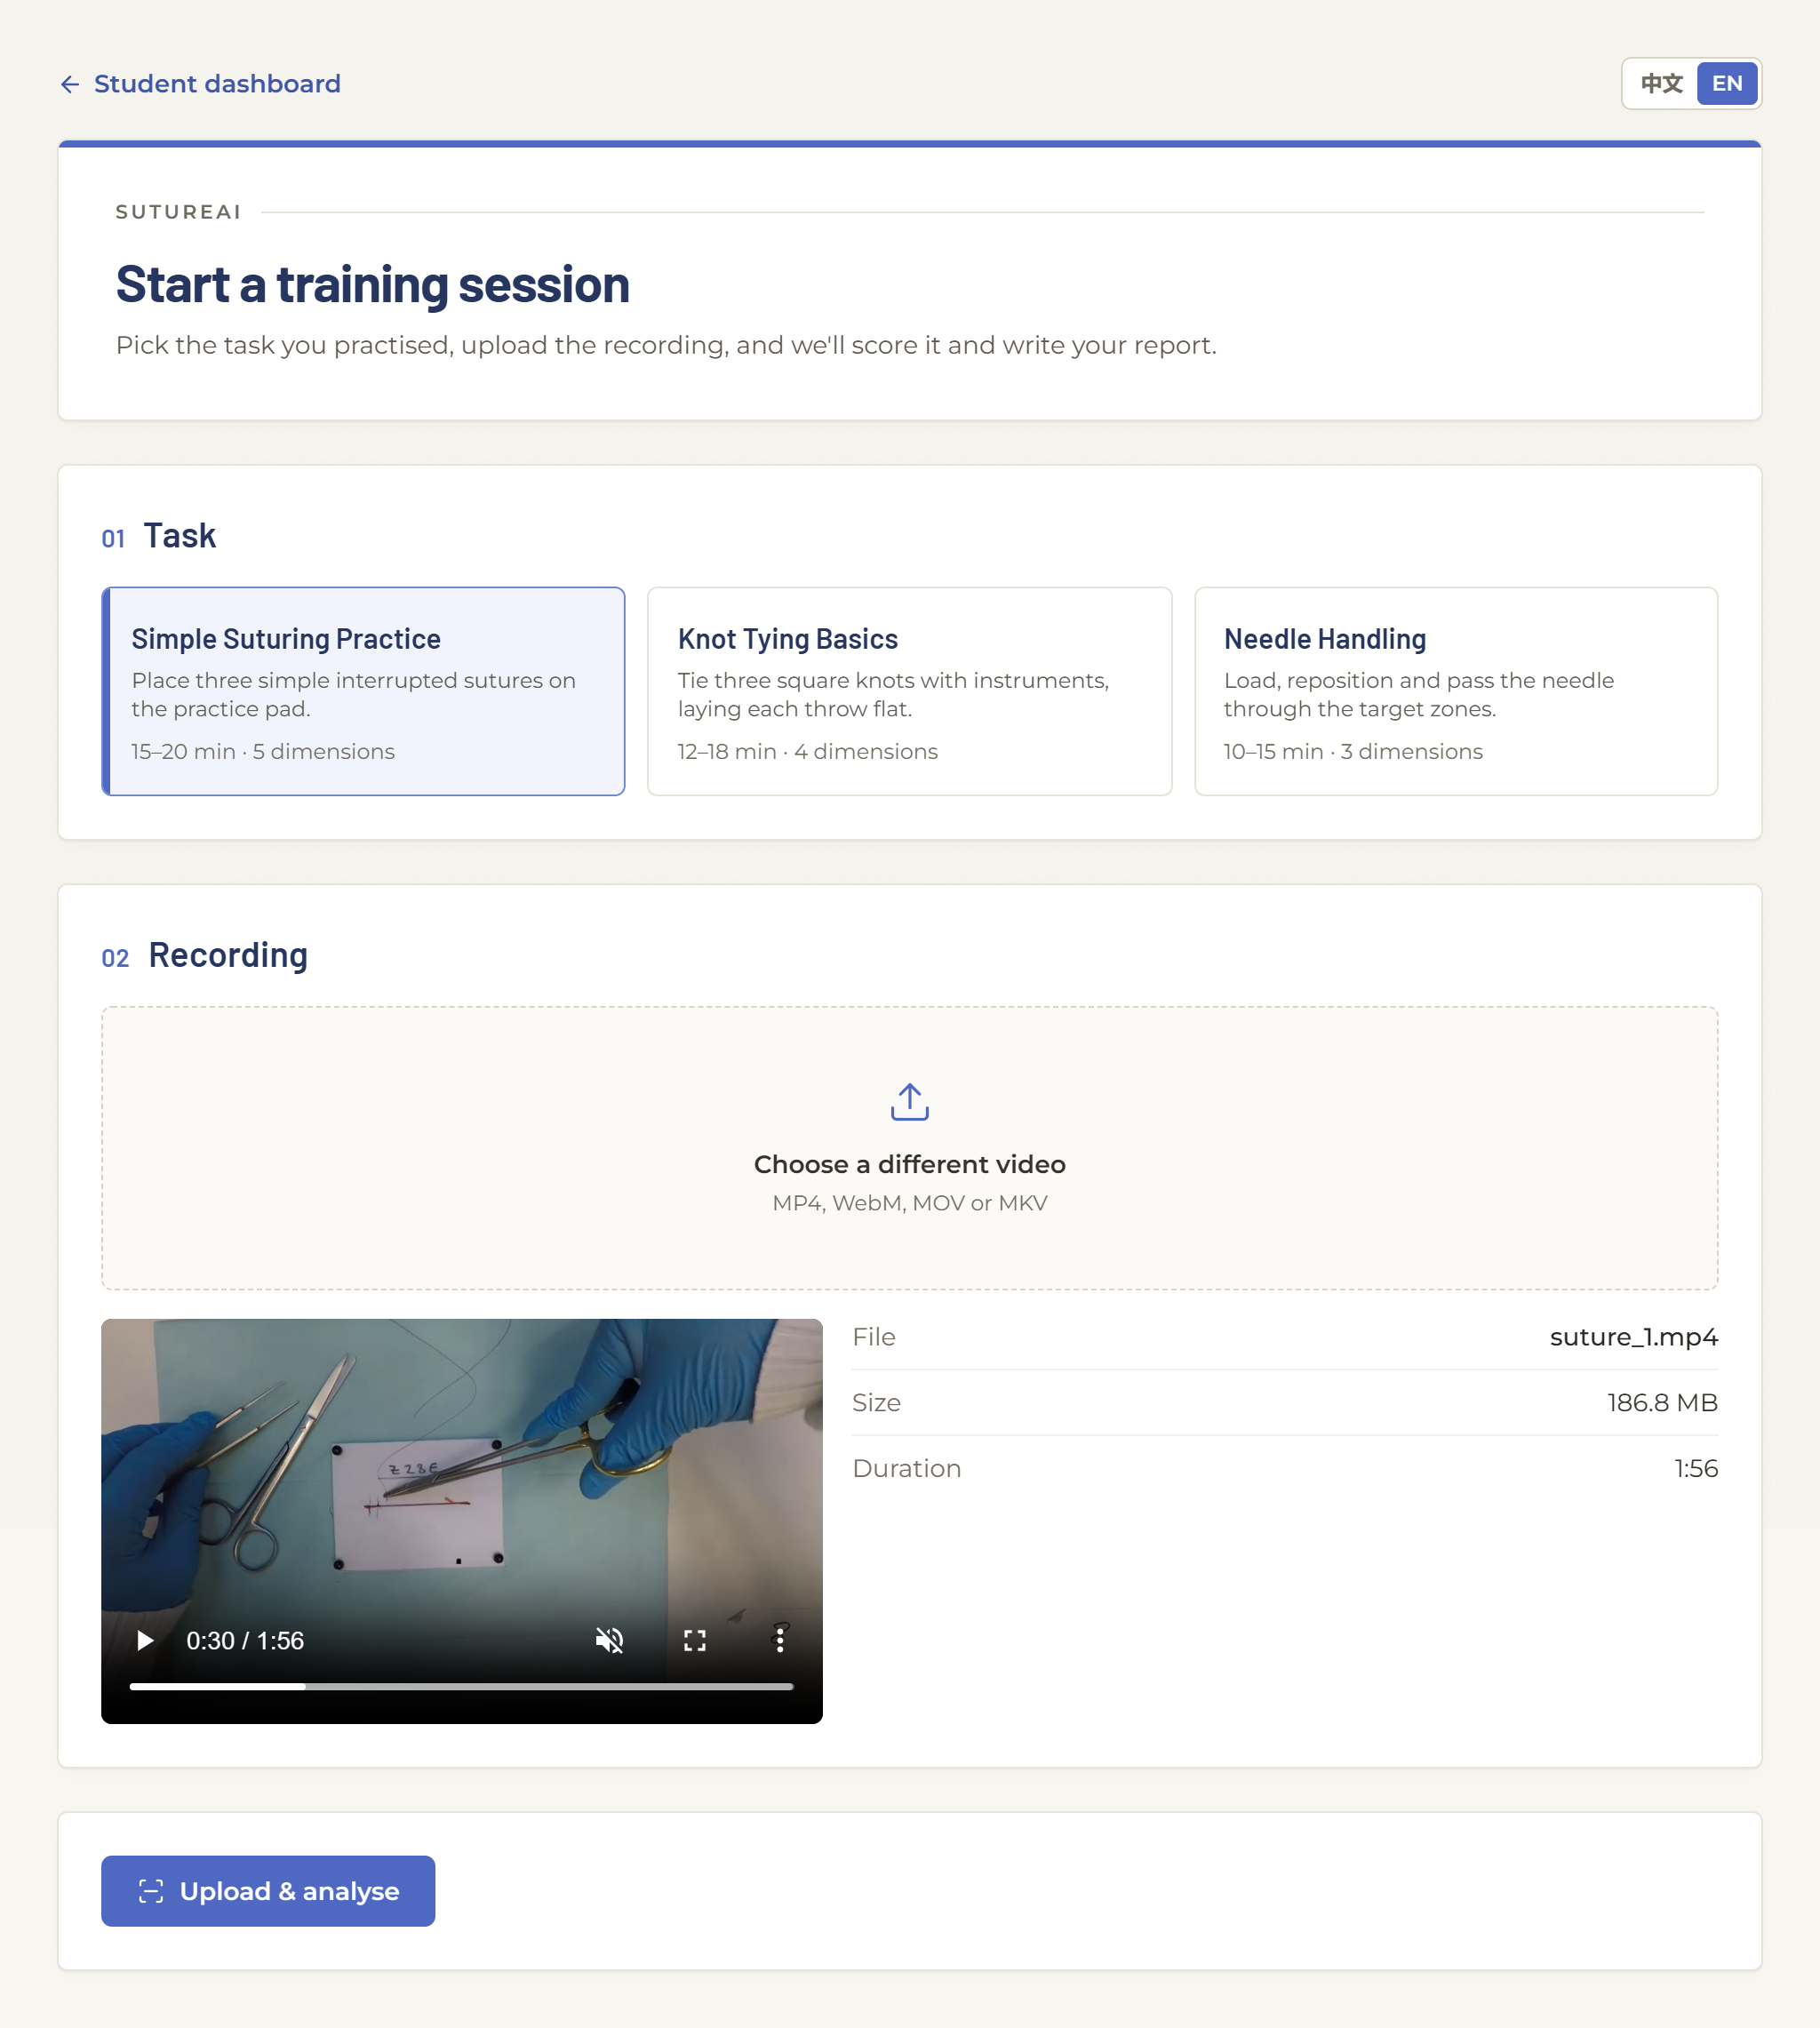
\includegraphics[width=\dimexpr\linewidth-2\fboxsep-2\fboxrule\relax]{figures/03-train-upload.png}}
\captionof{figure}{Choosing the task and the video before uploading.}
\end{minipage}

After the upload the page shows the analysis as it happens: a large percentage with an estimate
of the time left, a progress bar drawn as a line of stitches, a checklist of the seven analysis
stages (verify the recording, detect instruments, track hands, segment the procedure steps, score
the dimensions, write the report, link evidence clips) and a dark \emph{Activity} panel describing
what is being done right now. It usually takes under a minute. When it finishes, the report opens
automatically.

You can leave the page at any time: unfinished sessions are listed under \emph{Recordings in
progress} on your dashboard, and the page address (\page{/train/<session>}) can be reopened later.

\shot{04-train-processing.png}{Analysis in progress: percentage, stitch progress bar and stage
checklist on the left, live activity on the right.}

\begin{tip}
For the most reliable scores, film from above with the whole practice pad in frame, keep your
hands from covering the needle, use even lighting, and record the task from start to finish
without stopping.
\end{tip}

\subsection{Reading your report}
The header sheet of the report names the task, the student, the date and time, the task duration
and how confident the system is. The rotated stamp in the top-right corner shows whether your
instructor has looked at it yet: \emph{Pending review} or \emph{Reviewed} (hover over it for the
full wording). Use the \ui{Session} menu to switch between your reports and \ui{Export PDF} to save
one (Section~\ref{sec:export}).

Some reports then open with a \emph{Fix this first} tile: the single change that would gain you the
most points, why it matters, a drill to practise it and the moment it was seen. The numbered
sections follow.

\sect{01}{Overall performance}: the overall score drawn as a ring, with reliability, change
since your previous session, duration and dimension average. If your instructor confirmed a
different score, or accepted one of your appeals, a blue \emph{Current score} line shows the
score that counts. A \emph{Confidence notice} next to it lists anything that may limit the
accuracy of the scores. Where available, \emph{Where the points went} lists the biggest
losses first, next to your progress since the last session.

\sect{02}{Dimension scores}: a radar of the five dimensions and one card per dimension;
\ui{Metrics} shows the measurements behind a score.

\shot{05-report-overview.png}{Report header with the \emph{Reviewed} stamp, overall performance
and dimension scores.}

\sect{03}{Training timeline} lists what was detected and when: normal steps (hollow dot,
\emph{Step}), warnings (ochre, \emph{Warning}) and issues (brick red, \emph{Issue}). By default
only warnings and issues are shown; \ui{Show all \emph{n} events} adds the normal steps. \ui{Expand}
shows the detail; \ui{Replay} (or \ui{Jump}) plays the recording from that moment; on a report
without a recording the button reads \ui{View Clip}. Warnings
and issues also have an \ui{Appeal} link (Section~\ref{sec:appeal}). \emph{Assessment
highlights} beside it summarise the strongest dimension, the main issue, what to focus on
and the review status.

\shot{06-report-timeline.png}{Timeline. The struck-through issue at 01:05 was overturned after the
student's appeal; the warning at 00:47 can still be appealed.}

\sect{04}{Evidence replay} holds your recording. The marker strip under the video shows
every event (issues, warnings, steps); click a marker to jump there. Each key clip card's
\ui{Replay} button plays the recording from that moment.

\shot[0.86\linewidth]{13-report-evidence.png}{Evidence replay with the event marker strip and
the key clips.}

\sect{05}{Report feedback \& reflection} closes the report. On the left are the AI feedback
(blue tile), your strengths and areas for improvement (grey tiles) and recommended next steps
(dashed tile); on the right are your instructor's evaluation, your response and your personal
note (next section).

\subsection{Accepting or appealing your report}\label{sec:appeal}
If you agree with the report, press \ui{Accept report} in the \emph{Your response} tile of
section~05.

If you think a finding is wrong, \textbf{appeal it}:
\begin{enumerate}[label=\textbf{\color{brand}\arabic*.}]
  \item Find the warning or issue in the timeline (section~03) and press \ui{Replay} to check the
        moment yourself.
  \item Press \ui{Appeal} on that event and choose a reason: \emph{This didn't happen},
        \emph{The view was blocked}, \emph{Intentional / wrong moment} or \emph{Other}.
  \item Explain what really happened and press \ui{Send appeal}.
\end{enumerate}

\shot[0.72\linewidth]{14-appeal-form.png}{Appealing a finding directly from the timeline.}

The event then shows \chip[warn]{Appeal pending} and your instructor is notified. They watch the
clip and decide:
\begin{itemize}
  \item \textbf{Accepted}: the finding is struck through as \emph{Overturned after the student's
        appeal} and your score is raised (the chip shows by how much, e.g.\ \chip[good]{Appeal accepted · +2}).
  \item \textbf{Rejected}: the finding stays; your instructor explains why.
\end{itemize}
Either way the decision and the instructor's reasoning appear under \emph{Your response}. You can
withdraw an appeal while it is still pending, and you can also appeal the report as a whole with
\ui{Appeal the whole report}. A report can carry up to five appeals.

Above it, \textbf{Instructor evaluation} shows your instructor's final score, comment and teaching
focus once the review is complete. Below it, \textbf{Personal note} (dashed tile) is a private
reflection saved with the report with \ui{Save note}; instructors cannot see it.

{\setlength{\shotmax}{0.34\textheight}%
\shot[0.9\linewidth]{07-report-student-feedback.png}{Section 05 of a reviewed report: the appeal on
01:05 was accepted (+2) with the instructor's reasoning, and the student kept a private note.}}

\subsection{Exporting a report as PDF}\label{sec:export}
\begin{minipage}[t]{0.5\linewidth}
\vspace{0pt}
\raggedright\setlength{\parskip}{0.55em}
Press \ui{Export PDF} in the report header. A print layout opens in a new tab and the browser's
print dialog appears; choose \textbf{Save as PDF} as the destination. The PDF contains the summary,
what to fix first and where the points went, the dimension scores, the timeline with a still from
the recording at every event, strengths and next steps, all appeals with their decisions and the
instructor's review, so it can be filed as a record of the session.

The print page waits until the video stills have loaded. If the print dialog does not appear,
press \ui{Save as PDF} at the top of the page.
\end{minipage}\hfill
\begin{minipage}[t]{0.46\linewidth}
\vspace{0pt}
\centering
\fcolorbox{line}{white}{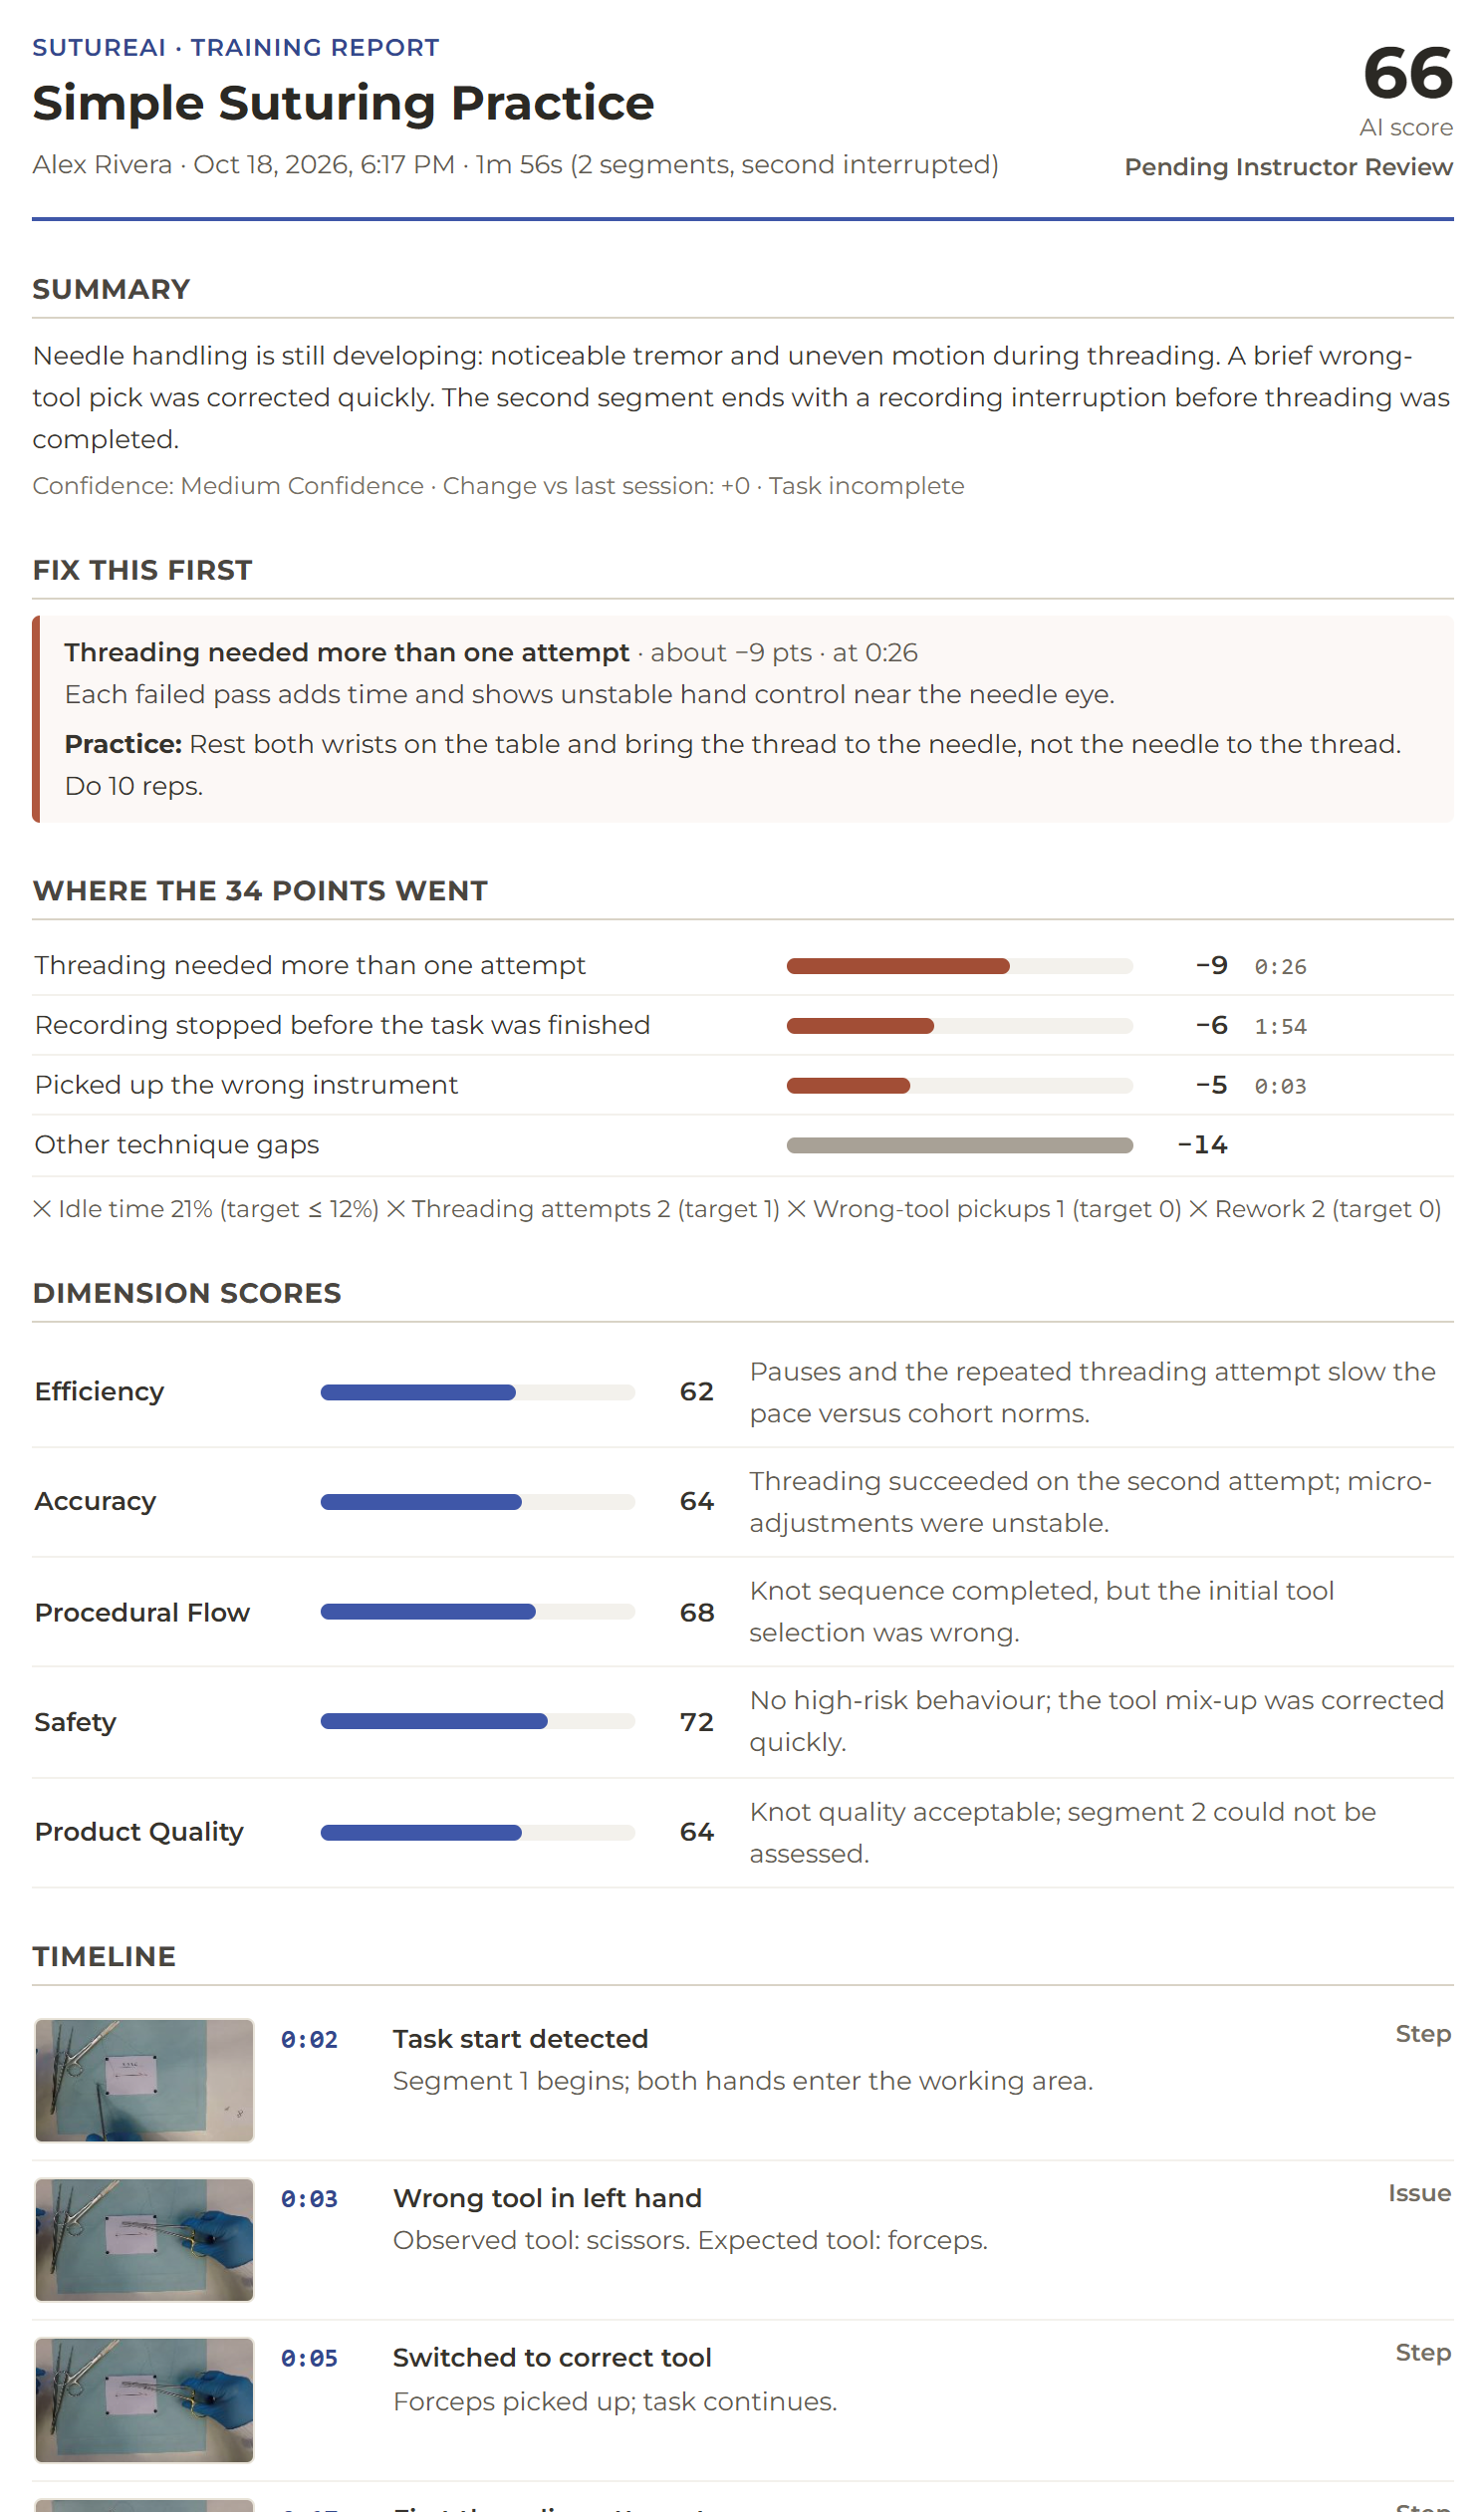
\includegraphics[width=\dimexpr\linewidth-2\fboxsep-2\fboxrule\relax]{figures/15-export-pdf.png}}
\captionof{figure}{Start of an exported report. Each timeline event shows the video frame at that moment.}
\end{minipage}

% ---- 4 instructors -------------------------------------------------------------
\section{For instructors}\label{sec:instructor}

The instructor area has two tabs in the top bar, \ui{Overview} and \ui{Review queue}; the language
switch, your name and \ui{Log out} sit on the right of the same bar. Both pages lead to student
pages and reports:

\begin{figure}[H]
\centering
\begin{tikzpicture}[node distance=0.55cm and 2.5cm]
  \node[box=brandeight] (ov) {\textcolor{brand}{\faThLarge}\\Class overview\\{\scriptsize\ttfamily\color{muted}/instructor}};
  \node[box=brandeight,right=of ov] (st) {\textcolor{brand}{\faIcon[regular]{user}}\\Student detail\\{\scriptsize\ttfamily\color{muted}/students/:id}};
  \node[box,right=of st] (rep) {\textcolor{brand}{\faIcon[regular]{file-alt}}\\Report\\(review form)};
  \node[box=brandeight,below=0.75cm of st] (q) {\textcolor{brand}{\faInbox}\\Review queue\\{\scriptsize\ttfamily\color{muted}/reviews}};
  \draw[arr] (ov) -- node[above,font=\scriptsize,color=muted]{click a name} (st);
  \draw[arr] (st) -- node[above,font=\scriptsize,color=muted]{Review / Open} (rep);
  \draw[arr] (q) -| node[pos=0.25,below,font=\scriptsize,color=muted]{Review / Decide} (rep);
  \draw[arr] (ov) |- node[pos=0.75,below,font=\scriptsize,color=muted]{KPI tiles} (q);
  \draw[arr] (ov.north) to[bend left=18] node[above,font=\scriptsize,color=muted]{Open report (needs attention)} (rep.north);
\end{tikzpicture}
\caption{Navigating the instructor area.}
\end{figure}

\subsection{Class overview}
Choose a group with the \ui{Cohort} menu at the top right; everything on the page refers to that
group.

\begin{itemize}
  \item \textbf{Key numbers}: students (and how many trained this week), sessions this week, the
        30-day average score, reports waiting for your review and open appeals. The last two are
        links into the review queue.
  \item \textbf{Needs attention} lists the students to look at now, most urgent first, each with a
        severity chip and a link to the student or the report.
  \item \textbf{Skill map} shows every student's recent average in each dimension on a blue scale.
        Paler cells are lower scores, so weak spots (for one student, or for the whole group in a
        column) stand out.
\end{itemize}

\shot{08-instructor-overview.png}{Class overview for Group A, below the instructor top bar.}

\begin{center}
\small
\begin{tabularx}{0.95\linewidth}{@{}l l Y@{}}
\toprule
\textbf{Flag} & \textbf{Level} & \textbf{When it appears} \\
\midrule
Open appeal & \chip[bad]{\faExclamationTriangle\ High} & The student appealed a finding and is waiting for your decision. \\
Declining scores & \chip[bad]{\faExclamationTriangle\ High} & The average of the last 3 reports is at least 8 points below the 3 before them. \\
Low score & \chip[warn]{\faIcon[regular]{clock}\ Medium} & The latest score is below 60. \\
Inactive & \chip[warn]{\faIcon[regular]{clock}\ Medium} & No training for 14 days or more, or never. \\
Failed upload & \chip[muted]{Low} & A recording could not be processed. \\
\bottomrule
\end{tabularx}
\end{center}

Below the skill map, the \textbf{Students} table lists everyone in the group. Click a column
heading to sort (by default the students with the most waiting work come first) or type in the
search box. \emph{Trend} is a small line of the last eight scores; \emph{Change} compares the
average of the last three reports with the three before them; \emph{To review} shows how many
reports and appeals are waiting for you.

\shot{09-instructor-roster.png}{Student roster.}

\subsection{Student detail}
Click a student's name anywhere to open their page: who they are, their group, current task and
focus, and their current flags; key numbers (latest score, reports, weakest dimension and what is
waiting on you); the overall score for every report (hover for details, click a point to open that
report); one small chart per dimension to see \emph{where} a change comes from; every session with
its review and response status; and the training calendar.

\shot{10-instructor-student.png}{A student whose scores are declining. The dimension charts show the
drop is broad rather than in one skill.}

\subsection{Review queue}
The queue collects reports from all your groups (or one, with the \ui{Cohort} filter) in three tabs,
each with its count:
\begin{itemize}
  \item \textbf{To review}: reports without a completed review, oldest first. Drafts stay here until completed.
  \item \textbf{Appeals}: reports with at least one appeal waiting for your decision.
  \item \textbf{Reviewed}: completed reviews, most recent first.
\end{itemize}
Each row ends with the action for that tab: \ui{Review}, \ui{Decide} or \ui{Open}.

\shot{11-review-queue.png}{The \emph{Appeals} tab of the review queue. Arrows such as \emph{74 $\rightarrow$ 72}
show a score you changed in a draft.}

\subsection{Reviewing a report}
Opening a report as an instructor turns its last section into \sect{05}{Report feedback \& review}:
the AI feedback on the left, \emph{Student appeals} on the right and the \emph{Instructor review}
form below.
\begin{enumerate}[label=\textbf{\color{brand}\arabic*.}]
  \item \textbf{Decide any appeals} under \emph{Student appeals}. Each one shows the disputed finding,
        the student's reason and message; when the report has a recording, the time button
        (e.g.\ \ui{\faPlay\ 0:03}) replays that moment. Choose \textbf{Accept --- overturn this finding}
        (the score is adjusted by the amount you set; a value is suggested: +4 for an issue, +2 for a
        warning) or \textbf{Reject --- keep the finding}, explain your decision, and press
        \ui{Send decision}.
  \item Set the \textbf{final score}. It starts at the AI score plus any accepted appeals; the
        \emph{Alignment} tile updates as you type.
  \item Write a \textbf{comment to the student} and add one or more \textbf{teaching focus} tags:
        type one and press Enter, or pick one of the suggested dimensions under the field.
  \item Press \ui{Save draft} to come back later (the student cannot see drafts), or
        \ui{Complete review} to send it. A completed review can still be edited with \ui{Update review}.
\end{enumerate}

\shot[0.9\linewidth]{12-review-form.png}{An appeal waiting for a decision, next to the AI feedback
and above the review form.}

\begin{center}
\small
\begin{tabularx}{0.8\linewidth}{@{}l Y@{}}
\toprule
\textbf{Alignment} & \textbf{Meaning} \\
\midrule
Agrees with AI & Final score equals the AI score. \\
Adjusted ($\le$10 pts) & Changed by 10 points or less. \\
Override (>10 pts) & Changed by more than 10 points. \\
\bottomrule
\end{tabularx}
\end{center}

If you accept an appeal after completing the review, the final score is adjusted automatically.

\begin{tip}
The \ui{View} switch in the report header toggles between \ui{Instructor} and \ui{As student sees
it}, which previews exactly what the student will see. Handy before completing a review.
\end{tip}

% ---- 5 reference ---------------------------------------------------------------
\section{Reference}\label{sec:reference}

\subsection{Session status}
\begin{figure}[H]
\centering
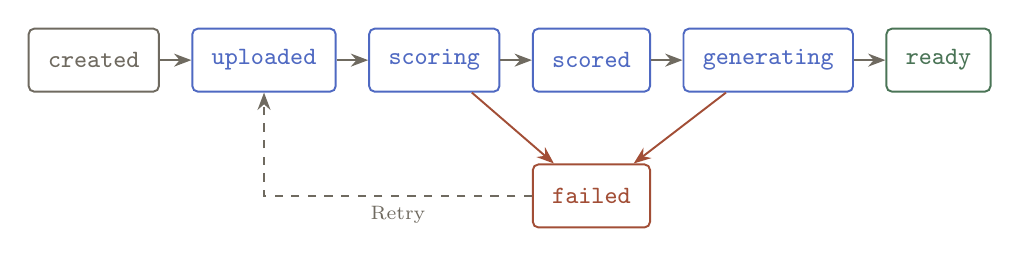
\begin{tikzpicture}[node distance=0.4cm]
  \node[state=muted] (c) {created};
  \node[state,right=of c] (u) {uploaded};
  \node[state,right=of u] (s) {scoring};
  \node[state,right=of s] (sd) {scored};
  \node[state,right=of sd] (g) {generating};
  \node[state=good,right=of g] (r) {ready};
  \node[state=bad,below=0.9cm of sd] (f) {failed};
  \foreach \a/\b in {c/u,u/s,s/sd,sd/g,g/r} \draw[arr] (\a) -- (\b);
  \draw[arr,color=bad] (s) -- (f);
  \draw[arr,color=bad] (g) -- (f);
  \draw[arr,dashed] (f.west) -| node[pos=0.25,below,font=\scriptsize,color=muted]{Retry} (u.south);
\end{tikzpicture}
\caption{Lifecycle of a training session. \emph{Retry} resumes from the last step that succeeded.}
\end{figure}

\begin{center}
\small
\begin{tabularx}{0.95\linewidth}{@{}l l Y@{}}
\toprule
\textbf{Status} & \textbf{Shown as} & \textbf{Meaning} \\
\midrule
\texttt{created} & Waiting for video & Session started, no video uploaded yet. \\
\texttt{uploaded} & Queued for analysis & Video received, waiting its turn. \\
\texttt{scoring} & Analysing video & The video is being analysed. \\
\texttt{scored} & Queued for report & Scores are ready; the report is waiting to be written. \\
\texttt{generating} & Writing report & The report is being written. \\
\texttt{ready} & Report ready & The report can be opened. \\
\texttt{failed} & Failed & Something went wrong; the page shows the reason and a \ui{Retry} button. \\
\bottomrule
\end{tabularx}
\end{center}

\subsection{Report and appeal status}
\begin{center}
\small
\begin{tabularx}{0.95\linewidth}{@{}l Y@{}}
\toprule
\textbf{Shown as} & \textbf{Meaning} \\
\midrule
Stamp \emph{Pending review} & Your instructor has not completed a review of this report yet. \\
Stamp \emph{Reviewed} & The review is complete; the instructor's evaluation is in section 05. \\
\chip[warn]{Appeal pending} & Sent; waiting for the instructor. The student can still withdraw it. \\
\chip[good]{Appeal accepted · +\emph{n}} & The finding is overturned and the score raised by \emph{n} points. \\
\chip[bad]{Appeal rejected} & The finding stands; the instructor's reasoning is shown. \\
\bottomrule
\end{tabularx}
\end{center}

\subsection{Troubleshooting}
\begin{description}[style=nextline,leftmargin=0pt,labelindent=0pt,labelwidth=0pt,font=\bfseries\color{brandeight}]
  \item[I cannot sign in.]
    Check the email address and password (the password is case-sensitive). If it still fails,
    ask your course administrator to check that your account exists.
  \item[My video is rejected.]
    Only MP4, WebM, MOV and MKV files are accepted, up to 1~GB by default. Empty files are refused.
  \item[Processing failed.]
    Open the session (from \emph{Recordings in progress} on the dashboard) and press \ui{Retry}.
    If it fails again, record a new session with better lighting and framing.
  \item[\ui{Accept report} is greyed out.]
    You have an appeal pending on that report. Wait for the decision or withdraw the appeal first.
  \item[There is no \ui{Appeal} link on an event.]
    Only warnings and issues can be appealed, each once, up to five appeals per report. Normal steps
    are hidden until you press \ui{Show all \emph{n} events}.
  \item[The print dialog did not open after \ui{Export PDF}.]
    Allow pop-ups for the site, or press \ui{Save as PDF} at the top of the print page once the
    video stills have loaded.
  \item[An instructor cannot see a student.]
    Instructors only see students in the groups they teach.
\end{description}

\end{document}
